\documentclass{article}
\usepackage[T1]{fontenc} % font encoding
\usepackage[utf8]{inputenc} % input encoding
\usepackage[ngerman]{babel} % set language
\usepackage{graphicx}
\usepackage{geometry}
\geometry{a4paper, top=25mm, left=20mm, right=25mm, bottom=30mm} 
\usepackage{caption}
\usepackage{amsmath}
\captionsetup{labelfont=it,labelsep=newline,singlelinecheck=false}
\usepackage{color}


\begin{document}
	
Nina Smeenk 366480\\
Martha Karpeter 367847

\section*{Exercise Sheet 6}
\subsection*{Exercise 1}

Polarizing the statement in the exercise will yield the following:\\
Consider a non-deg., non-empty Conic in $\mathbb{R}P^2$, four points $t_A,t_B,t_C,t_D$ on the conic and their corresponding tangents $A,B,C,D$.\\
Define the lines $P=\overline{t_A t_B},Q=\overline{t_B t_C}, R=\overline{t_C t_D}, S=\overline{t_D t_A}$.\\
Then the four points $PR=P\cap R, QS=Q\cap S,AC=A \cap C$ and $BD=B \cap D$ are collinear.
\begin{center}
	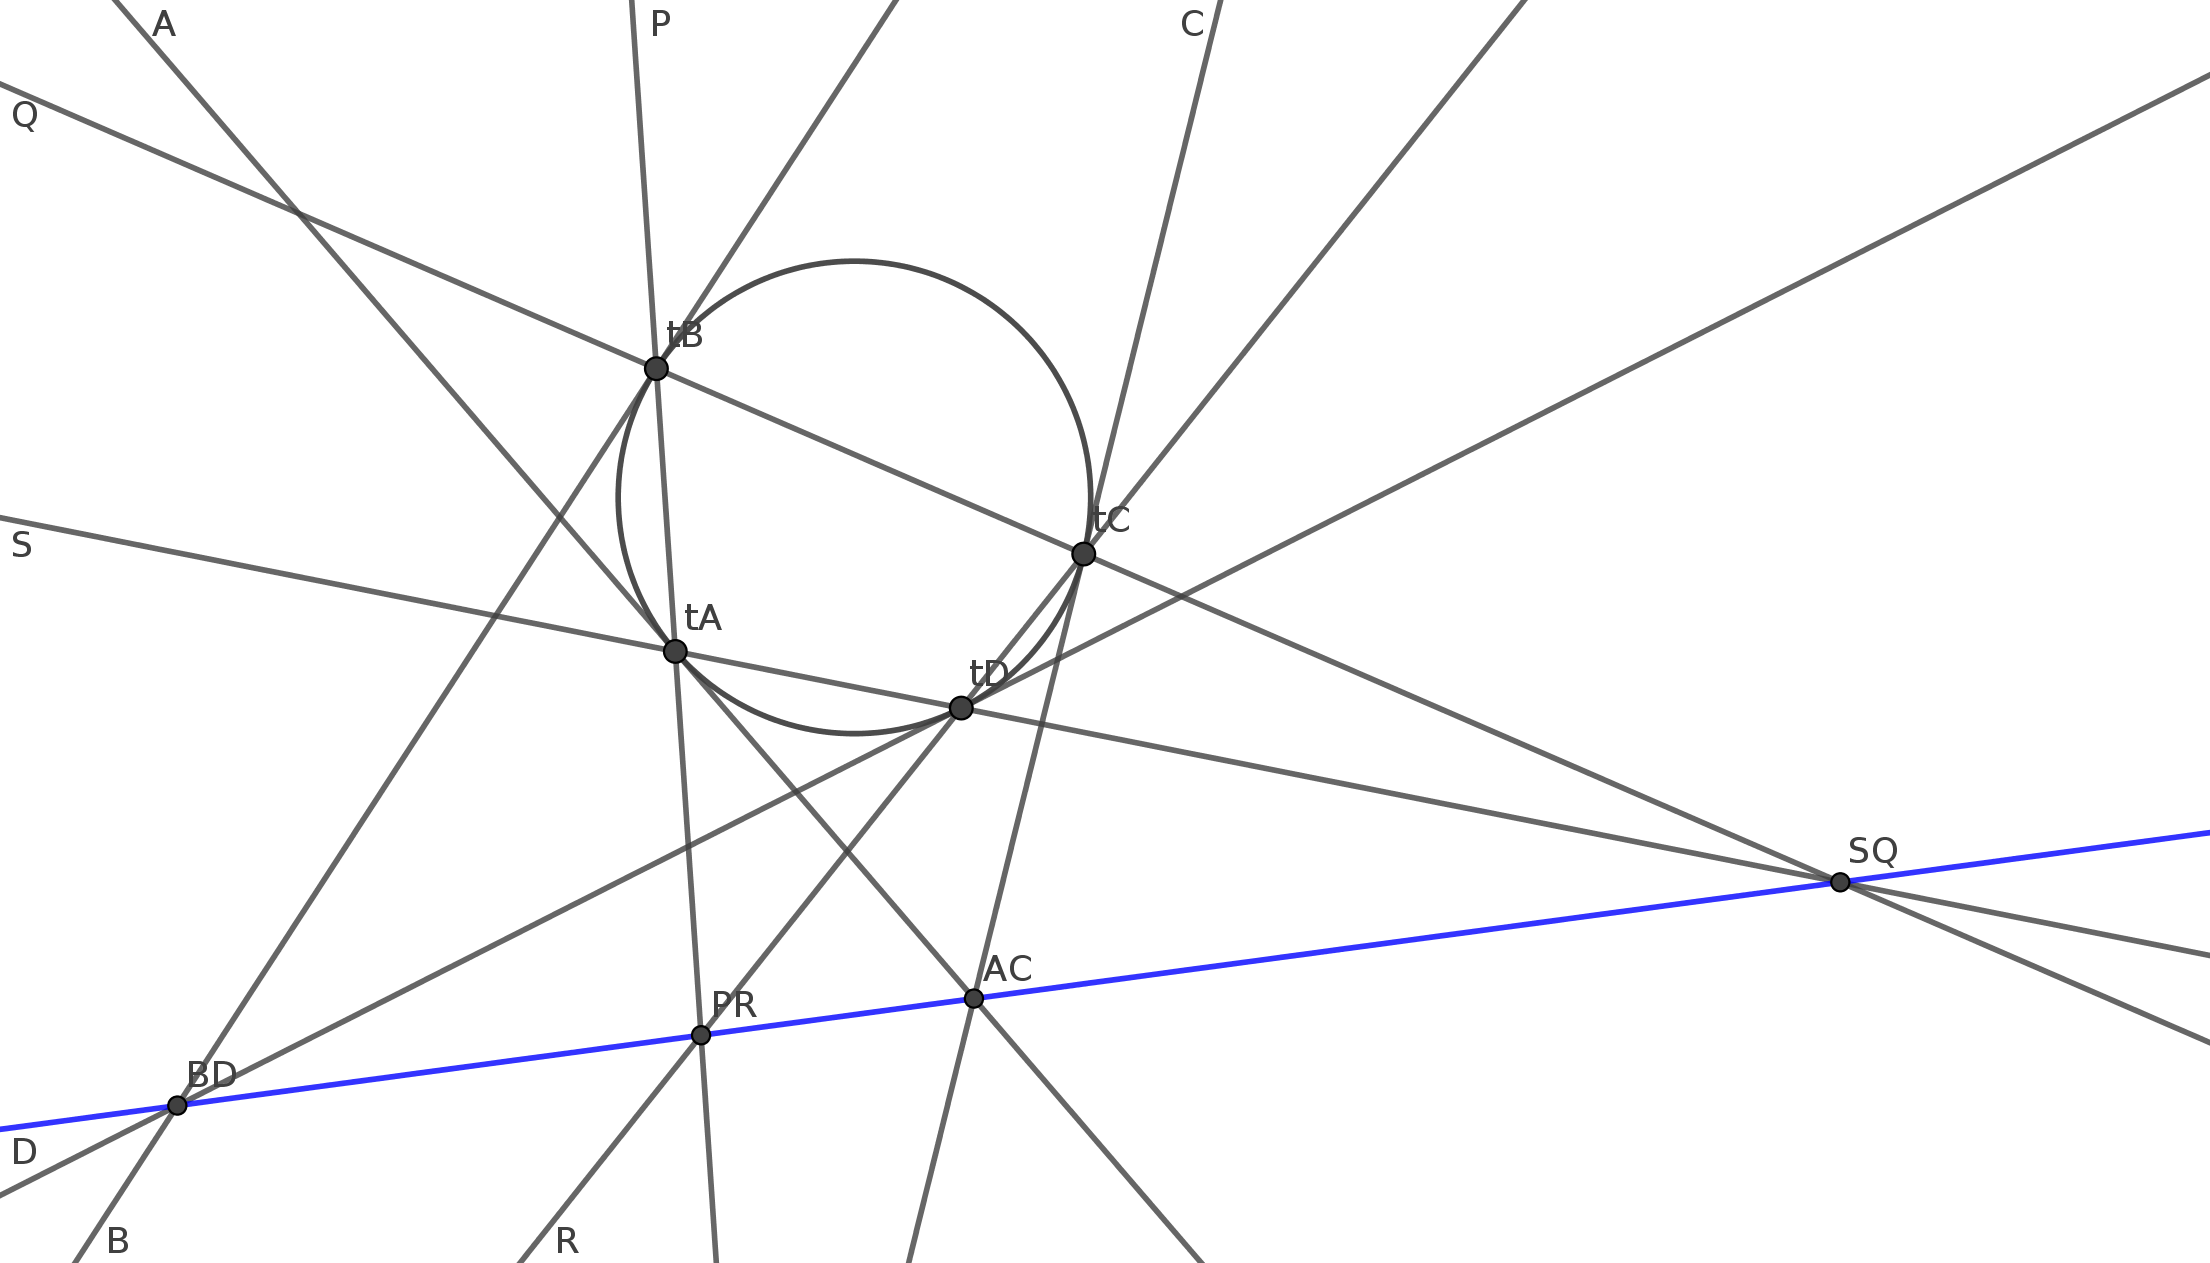
\includegraphics[width=13cm]{Hausaufgabe_05_01_Dual}
\end{center}

	

\end{document}
